\documentclass{article}

% Language setting
% Replace `english' with e.g. `spanish' to change the document language
\usepackage[english]{babel}
\usepackage{float} 

% Set page size and margins
% Replace `letterpaper' with `a4paper' for UK/EU standard size
\usepackage[letterpaper,top=2cm,bottom=2cm,left=3cm,right=3cm,marginparwidth=1.75cm]{geometry}
% Useful packages
\usepackage[round]{natbib}
\bibliographystyle{apalike}
\usepackage{amsmath}

\usepackage{graphicx}
\usepackage{subcaption}
\usepackage[colorlinks=true, allcolors=blue]{hyperref}

\title{\textbf{Correlation Analysis on Cryptocurrency and Traditional Financial Assets}}
\author{Yujie Tao
\\Zihan Liu
\\Wenqian Yang}

\begin{document}
\maketitle

\begin{abstract}
Currently, research on the dynamic relationship between cryptocurrency and traditional financial asset markets is limited and has yet to reach a consensus. This project empirically examines the dynamic correlations among Bitcoin, the S\&P 500 Index, COMEX gold futures, and WTI crude oil futures within a unified framework, using daily trading data from November 2021, to December 2024.
This study tries to address a gap in existing research by systematically investigating the time-varying relationships between typical cryptocurrencies and traditional financial asset markets within a single framework. The study aims to improve the understanding of cryptocurrencies within modern financial assets and has significant implications for policymakers and investors alike.
\\
\textbf{Keywords}: cryptocurrency; financial assets; correlation analysis

\end{abstract}

\section{General View}

In general, bitcoin shows a moderate positive correlation with the S\&P 500 Index, while its relationships with COMEX Gold Futures and Aggregate Oil Futures are weaker and more variable. Traditional assets like gold and oil futures show a moderate positive correlation, reflecting shared macroeconomic influences.

In what follows in this report, we first compose a rather detailed literature review on the related topic and then display and explain some findings from our own research.
\section{Significance}
Due to the unique anonymity characteristics, cryptocurrencies are highly susceptible to asset price bubbles, and the contagion of such bubbles poses risks to the stability of the financial system. In fact, the anonymity of cryptocurrency users and the absence of intermediary institutions result in low transaction costs, making cryptocurrencies an attractive medium of exchange for potential users \cite{baur2018b}. However, cryptocurrencies are also characterized by high volatility \cite{chu2017,katsiampa2017}, heavy tails \cite{osterrieder2017,gkillas2018,phillip2018}, and leverage effects \cite{phillip2018}, distinguishing them as a new asset class rather than a traditional medium of exchange \cite{yermack2015,baek2015,dyhrberg2016b}. Many investors now view cryptocurrencies as alternative assets or diversification tools to reduce portfolio risk \cite{tiwari2019}. However, the cryptocurrency market remains less developed compared to traditional financial markets, and investor understanding of cryptocurrencies may not be entirely accurate. Consequently, the relationships between price volatility and risk spillovers between cryptocurrency and traditional financial markets are not yet fully understood.
This study’s examination of the correlation between cryptocurrency and traditional financial asset markets holds critical implications for policymakers and investors. Understanding the evolving relationship between cryptocurrencies and traditional financial assets can help policy makers formulate appropriate regulations to prevent contagion effects and protect financial stability. For investors, assessing the risk spillovers and hedging effectiveness of cryptocurrencies against traditional financial assets enables the selection of the most efficient cryptocurrency for hedging purposes and the evaluation of optimal hedging strategies.

\section{Literature Review}

\subsection{Studies on Price Volatility and Spillover Effects in the Cryptocurrency Market}
\cite{mensi2019cryptocurrency} use wavelet coherence and cross-wavelet transform methods to examine the interconnectedness among Bitcoin and five major cryptocurrencies (Dash, Ethereum, Litecoin, Monero, and Ripple) and the impact on portfolio risk. \cite{sifat2019} apply vector error correction models (VECM), Granger causality tests, autoregressive moving average (ARMA), and autoregressive distributed lag (ARDL) models to explore the leading and lagging price relationship between Bitcoin and Ethereum, concluding that they mutually influence each other. \cite{katsiampa2019} utilize diagonal BEKK and asymmetric diagonal BEKK models on intraday data of eight cryptocurrencies to investigate conditional volatility and covolatility among major cryptocurrencies, finding high volatility and strong interdependencies within the market.

\subsection{Studies on Price Volatility and Spillover Effects in Traditional Financial Markets}
\cite{mensi2021oil} analyze the spillover effects and correlations between crude oil futures and various maturities in the European Bond Market (EBM), further assessing the hedging effectiveness of oil-bond portfolios during calm and turbulent periods. \cite{sun2021spillover} examine spillover effects between the China oil and stock markets at different time frequencies based on the trading frequency, finding that the role of stocks as the main source of volatility varies across time domains. \cite{peng2020dynamic} employ linear and non-linear Granger causality tests in combination with bivariate empirical model decomposition to evaluate multi-scale dynamic interactions and volatility effects between the China stock market and the global oil market.

\subsection{Studies on Price Volatility and Spillover Effects Between Cryptocurrencies and Traditional Financial Markets}

Although various scholars have explored the dynamic relationship between cryptocurrencies and traditional financial assets, consensus remains elusive. \cite{dyhrberg2016b} find a strong correlation between cryptocurrency and stock markets. \cite{akyildirim2020relationship} identify a time-varying positive correlation between the conditional correlation of cryptocurrencies and financial market stress. They concluded that cryptocurrencies transmit risk to traditional financial assets, and different cryptocurrencies exhibit similar spillover patterns to traditional financial markets at specific times.

In contrast, \cite{corbet2019cryptocurrencies} and \cite{baur2018b} find that cryptocurrencies remain relatively isolated from traditional financial markets. \cite{baur2018b}, \cite{briere2015virtual}, and \cite{bouri2018bitcoin} argue that the correlation between cryptocurrencies and bonds or stocks is very low, suggesting that cryptocurrencies can serve as a diversification tool. Further studies by \cite{dyhrberg2016b}, \cite{bouri2018bitcoin}, and \cite{bencheikh2020asymmetric} demonstrate that cryptocurrencies exhibit some hedging capabilities relative to traditional financial assets. \cite{yermack2015} suggest that the combination of gold and Bitcoin can serve as a hedging strategy.




In summary, in the literature it is well recognized that cryptocurrencies and traditional financial asset markets exert impact on each other to various extents in terms of magnitude; the combination of both might help investors to diversify risks. 



\section{Data}


This study aims to investigate the relationship between the cryptocurrency market and traditional financial asset markets. For the cryptocurrency market, we initially considered the major cryptocurrencies with high market capitalization. To ensure data representativeness and continuity, we focused on cryptocurrencies with active trading and notable volatility between 2021 and 2024, including Bitcoin, Ethereum, and Ripple. After further screening, Bitcoin was chosen as the primary representative of the cryptocurrency market, as it has consistently maintained a dominant market share (more than 60\% of the total market capitalization) and its price trends tend to reflect broader market movements in cryptocurrency. This selection ensures both the representativeness of the study and avoids data issues that smaller or recently launched cryptocurrencies might present.

In terms of traditional financial assets, global oil prices currently refer to oil futures, with West Texas Intermediate (WTI) crude serving as a major global benchmark. The price movements of WTI often set the trend for other oil varieties. The US stock market, as one of the most influential capital markets worldwide, is represented by the S\&P 500 Index, which includes more than 500 publicly traded companies in various industries and is widely recognized as a suitable indicator of global stock market performance. Additionally, the gold futures market is a key component of the global financial market, and the COMEX gold futures, which are part of the New York Mercantile Exchange, are particularly influential, with the International Monetary Fund (IMF) and the US Treasury Department also trading on this exchange. COMEX gold futures often play a decisive role in global gold price trends. Consequently, this study uses the daily closing prices of the S\&P 500 Index, COMEX gold futures, and WTI crude oil futures to represent traditional financial asset market trends.
 
The data showing in Figure~\ref{price}  for this study cover daily closing prices from December 2021 to November 2024, totaling approximately 754 trading days.

To measure the daily returns of these assets, this study defines daily returns as the first-order logarithmic difference between closing prices on consecutive trading days. If $P_t$  represents the closing price at time t, then the daily return $Rt$ is defined as $R\_t = (\ln Pt - \ln P_{t-1}) \times 100\%$. 

\begin{figure}
    \centering
    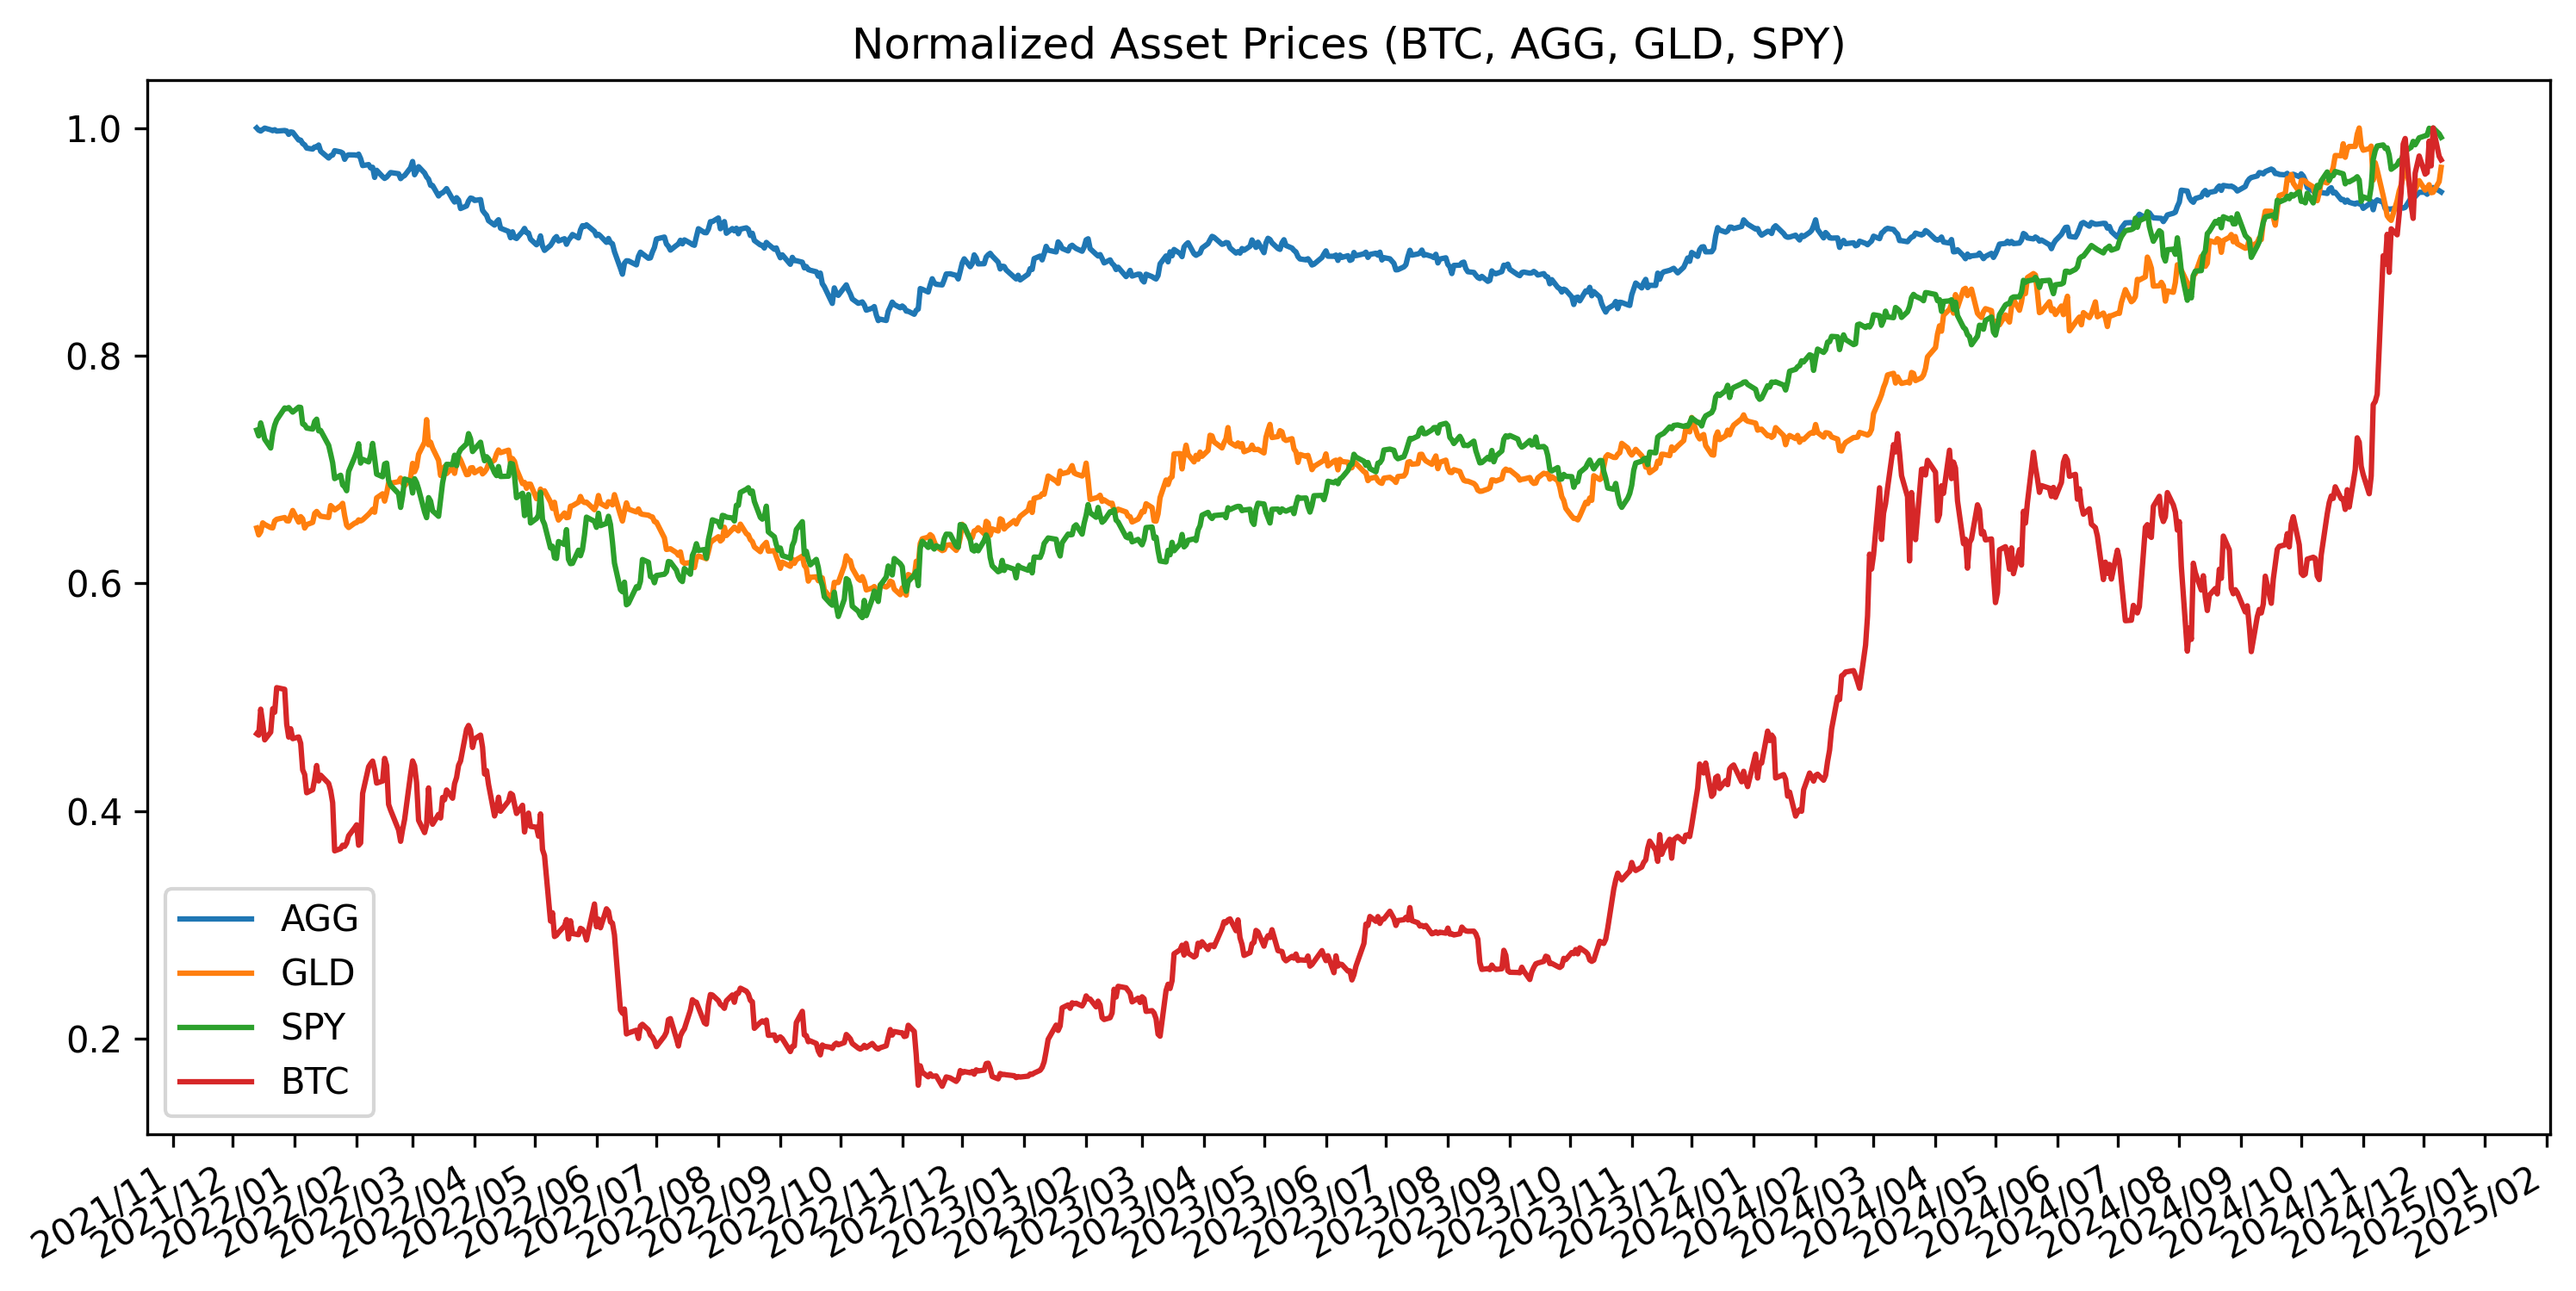
\includegraphics[width=1\linewidth]{figure/normalized_asset_prices.png}
    \caption{Normalized Price}
    \label{price}
\end{figure}


\section{Results and Findings}





In this section, we report our main findings accompanied by some visualization figures.

\subsection{Short-term Correlation Analysis by Pearson (linear)}



\begin{figure}
    \centering
    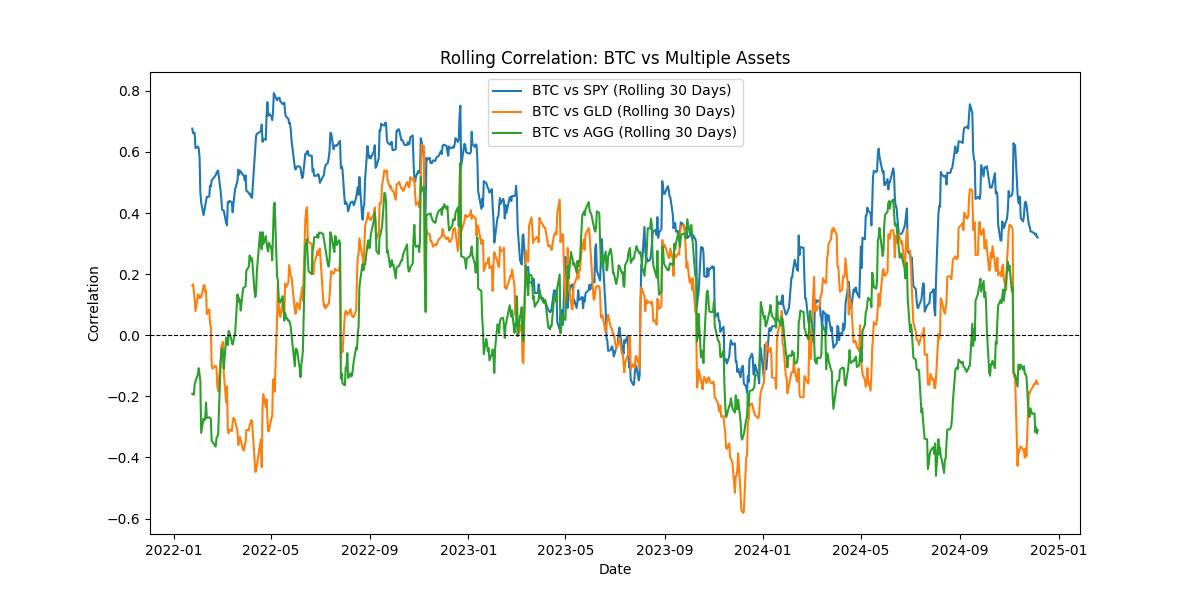
\includegraphics[width=1\linewidth]{figure/rolling_correlation_multi.png}
    \caption{Correlation Analysis}
    \label{volatility}
\end{figure}


We analyze the correlations between Bitcoin and other major financial assets, focusing on both dynamic and static perspectives. Figure~\ref{volatility} illustrates the rolling 30-day correlation between Bitcoin and the S\&P 500 Index, COMEX Gold Futures and Aggregate Oil Futures from January 2022 to December 2024, this is more focus on the short-term relationship, as the window is 30 days. From the results, we found Bitcoin’s correlation with the S\&P 500 Index remains predominantly positive, frequently ranging between 0.3 and 0.7, suggesting moderate alignment with equity markets and reflecting its behavior as a risky high-beta asset. Peaks near 0.7 indicate an increase in comovement, likely driven by macroeconomic events that affect both equities and cryptocurrencies. In contrast, the correlation of Bitcoin with COMEX Gold Futures shows substantial variability, oscillating between weakly negative and weakly positive values. Dips below -0.2 during early and late 2022 reflect instances where Bitcoin and gold likely acted as opposing risk hedges, while occasional positive correlations indicate alignment during broader economic shifts. The relationship of Bitcoin with aggregate oil futures is similarly inconsistent, with correlations fluctuating between -0.4 and 0.3, reflecting idiosyncratic shocks in the energy sector or the cryptocurrency market.


\subsection{Long-term Correlation Analysis by LSTM and VAR (no-linear)}

In this section, we conduct the Vector Autoregression Model and the LSTM-based model to analyze and extract relationships between financial assets using time series data, different from the Pearson correlation analysis we use these 2 nonlinear analyses and focus more on the long term effects. 

\subsubsection{Vector Autoregression (VAR) Model}

The vector autoregression (VAR) model is a powerful statistical tool used to capture the interdependencies and dynamics between multiple time series. In this study, the VAR model was applied to evaluate the causal relationships between Bitcoin (BTC) and traditional financial assets, including the S\&P 500 Index (SPY), COMEX Gold Futures (GLD), and Aggregate Bond Index (AGG). By using Granger causality tests within the VAR framework, we aimed to determine whether movements in traditional assets could predict Bitcoin's price dynamics or vice versa.

The Granger causality test results, shown at Figure~\ref{var}, indicate no significant causal relationship between BTC and the selected traditional assets at the 5\% significance level. For AGG, GLD, and SPY, the p-values (0.977, 0.423, and 0.091, respectively) are above the critical threshold of 0.05, leading us to fail to reject the null hypothesis that these assets do not Granger-cause Bitcoin. This suggests that historical movements in these traditional assets do not provide predictive power for Bitcoin's price behavior. This finding aligns with the results obtained from the LSTM model, which also demonstrated that Bitcoin exhibits little to no correlation with traditional assets over the long term. Together, these analyses reinforce the perception of Bitcoin as an independent asset class, largely unaffected by the factors driving traditional financial markets.


\begin{figure}
    \centering
    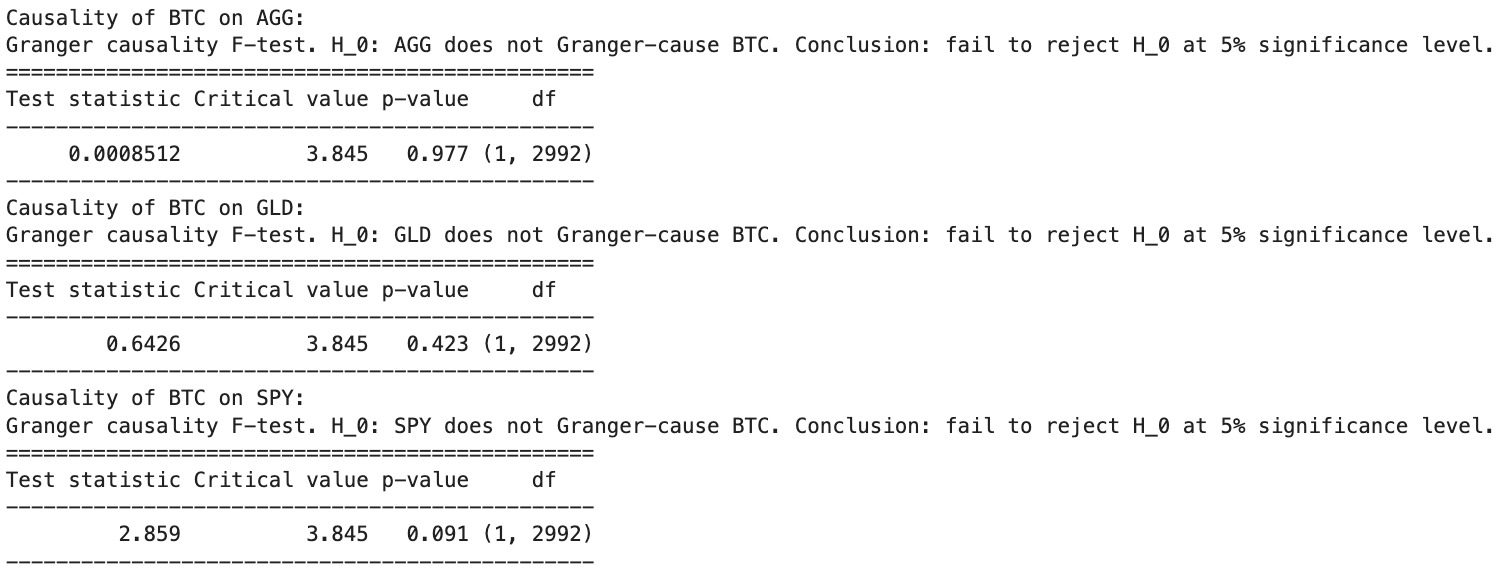
\includegraphics[width=1\linewidth]{figure/var.png}
    \caption{Causality of BTC on tradional assets}
    \label{var}
\end{figure}


\subsubsection{Long Short-Term Memory Model}

\begin{figure}
    \centering
    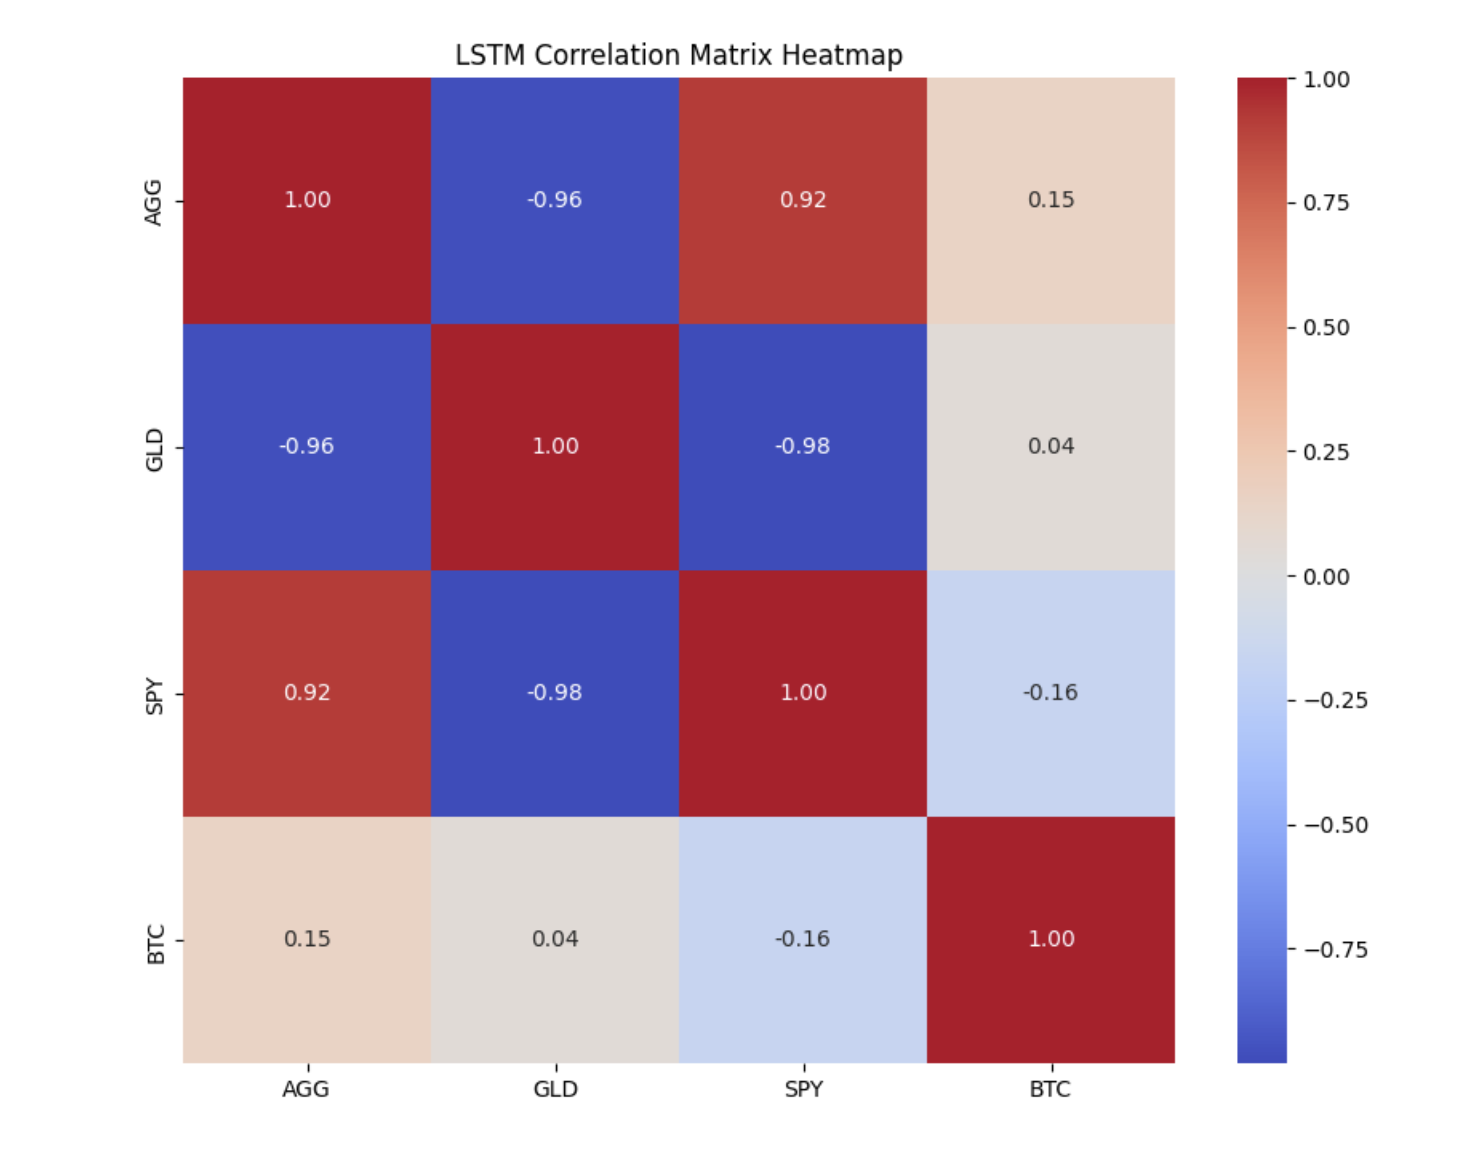
\includegraphics[width=0.7\linewidth]{figure/lstm_correlation_heatmap_with_labels.png}
    \caption{LSTM Heatmap}
    \label{lstmh}
\end{figure}

Figure~\ref{lstmh} The LSTM correlation heatmap reveals that Bitcoin (BTC) exhibits very low correlations with traditional financial assets such as the SP 500 Index (SPY), COMEX Gold Futures (GLD), and Aggregate Bond Index (AGG). For example, the correlation between BTC and SPY is -0.16, while its correlation with GLD and AGG is 0.04 and 0.15, respectively. These values suggest that Bitcoin's price movements are largely independent of traditional markets, aligning with the narrative that Bitcoin functions as an alternative asset class. Unlike stocks, bonds, or gold, Bitcoin’s price dynamics are often influenced by cryptocurrency-specific factors, such as regulatory developments, blockchain adoption, and speculative market behavior, rather than macroeconomic indicators that traditionally drive these assets.

In contrast to the earlier Pearson correlation analysis, which may have shown higher correlations in certain short-term market conditions, the LSTM heatmap reflects Bitcoin’s longer-term independence from traditional assets. By sequentially processing data and capturing temporal dependencies, the LSTM model provides a deeper understanding of how Bitcoin’s price movements deviate from broader market trends over time. The differences between the two methods underline the importance of using advanced models like LSTM to uncover nuanced relationships that linear correlations might overlook.

\section{Conclusion}

This project explored the relationships between Bitcoin (BTC) and traditional financial assets, including the S\&P 500 Index (SPY), COMEX Gold Futures (GLD), and Aggregate Bond Index (AGG), using Pearson correlation, Vector Autoregression (VAR) analysis, and Long Short-Term Memory (LSTM) modeling. Each method provided distinct insights into the nature of these relationships.

The Pearson correlation analysis highlighted that Bitcoin generally exhibits low or negligible correlations with traditional assets over time, reinforcing its reputation as an alternative and independent asset class. This independence suggests Bitcoin's potential as a diversification tool in investment portfolios. The VAR model, through Granger causality tests, further confirmed the lack of predictive relationships between traditional asset price movements and Bitcoin. The p-values obtained for AGG, GLD, and SPY consistently failed to reject the null hypothesis, indicating no significant causal influence of traditional assets on Bitcoin's price behavior.

The LSTM model, leveraging its ability to capture non-linear dependencies and temporal patterns, provided complementary results. It also demonstrated low long-term correlations between Bitcoin and traditional assets, further validating Bitcoin’s unique position in the financial ecosystem. The consistency of findings across these methodologies underscores Bitcoin's distinction as a separate asset class, driven by cryptocurrency-specific factors rather than the macroeconomic variables that influence traditional markets.

In conclusion, the combined results from Pearson correlation, VAR, and LSTM analyses confirm Bitcoin's role as an independent asset with limited connection to traditional financial assets. While its distinct behavior offers opportunities for diversification, it also presents challenges for integration into conventional risk and portfolio management frameworks, requiring careful consideration by investors and policymakers alike.




\newpage
\bibliographystyle{plain}
\bibliography{Bibliography}
\end{document}
